\documentclass[11pt,a4paper]{article}

\usepackage[utf8]{inputenc}
\usepackage[margin=1in]{geometry}
\usepackage{graphicx}
\usepackage{booktabs}
\usepackage{tabularx}
\usepackage{xcolor}
\usepackage{titlesec}
\usepackage{listings}
\usepackage{amsmath,amssymb}
\usepackage{hyperref}
\usepackage{fancyhdr}
\usepackage{enumitem}

\hypersetup{
    colorlinks=true,
    linkcolor=blue!70!black,
    citecolor=blue!70!black,
    urlcolor=blue!70!black
}

\pagestyle{fancy}
\fancyhf{}
\rhead{\textcolor{gray}{NoSQL Project Analysis Assignment}}
\lhead{\textcolor{gray}{FraudShield: Multi-Model NoSQL Engine}}
\cfoot{\thepage}

\titleformat{\section}{\large\bfseries\color{blue!70!black}}{\thesection.}{0.5em}{}[\titlerule]
\titleformat{\subsection}{\normalsize\bfseries\color{black!80}}{\thesubsection}{0.5em}{}

\lstset{
    basicstyle=\small\ttfamily,
    backgroundcolor=\color{gray!10},
    frame=single,
    rulecolor=\color{gray!40},
    breaklines=true,
    keywordstyle=\color{blue!80!black}\bfseries,
    commentstyle=\color{green!50!black}\itshape,
    stringstyle=\color{red!70!black},
    showstringspaces=false,
    tabsize=2
}

\begin{document}

\begin{center}
    {\LARGE \textbf{NoSQL Project Analysis Assignment}}\\[0.4em]
    {\large \textbf{FraudShield: Real-Time Multi-Model NoSQL Fraud Detection Framework}}\\[0.2em]
    {\small \textit{Technical Specification, Architecture, and Data Model Proposal}}\\[1em]
\end{center}

\vspace{-0.5em}
\hrule
\vspace{1em}

% -------------------------------------------------------------
\section{Personal and Contact Details}

\begin{table}[h!]
\centering
\renewcommand{\arraystretch}{1.3}
\begin{tabularx}{\textwidth}{|l|X|}
\hline
\textbf{Student Name} & Sarthak Gupta \\ \hline
\textbf{Enrolment Number} & 2427010032 \\ \hline
\textbf{Section} & Section J \\ \hline
\textbf{Subject Name} & NoSQL Databases \\ \hline
\textbf{Email Address} & sarthak.2005gupta@gmail.com \\ \hline
\textbf{Contact No:} & 9599301499 \\ \hline
\end{tabularx}
\end{table}

% -------------------------------------------------------------
\section{Project Domain / Classification}
\noindent \textit{Identify the technical domain and application area of your proposed project. (20-40 Words):}

\vspace{0.4em}
\noindent Financial Technology (FinTech), Distributed NoSQL Data Engineering, and Real-Time Graph Intelligence. The project focuses on high-throughput financial fraud ring detection, money laundering path identification, and polymorphic transaction auditing. \textit{(31 words)}

% -------------------------------------------------------------
\section{Project Title}
\noindent \textbf{FraudShield: A Multi-Model NoSQL Framework for Real-Time Financial Fraud Ring Identification and Polymorphic Transaction Auditing}

% -------------------------------------------------------------
\section{Problem Statement}
\noindent \textit{Explain the existing challenges and why the problem requires an efficient data management solution. (50-70 Words):}

\vspace{0.4em}
\noindent Modern digital payment ecosystems process tens of thousands of heterogeneous transactions per second. Organized cybercriminal syndicates bypass traditional relational database rules by utilizing complex multi-hop mule networks, circular fund routing, and synthetic identities across shared device clusters. Traditional relational databases fail due to exponential join latency on deep recursive queries and rigid schemas unable to ingest polymorphic payment payloads with sub-second latency. \textit{(65 words)}

% -------------------------------------------------------------
\section{Proposed Solution}
\noindent FraudShield implements a high-throughput, low-latency multi-model NoSQL architecture combining \textbf{Document NoSQL (MongoDB)} and \textbf{Graph NoSQL (Neo4j / Property Graph Engine)} to ingest, index, and analyze financial transactions in real time:

\begin{itemize}[leftmargin=1.5em]
    \item \textbf{Type of NoSQL Databases Proposed:} Multi-model system utilizing Document Store (MongoDB) and Graph Store (Neo4j / Property Graph Engine).
    \item \textbf{Reason for Selection:} MongoDB provides flexible BSON schemaless storage, write-optimized sharding, and fast secondary indexing. Neo4j delivers index-free adjacency ($O(1)$ traversal per hop) enabling millisecond cycle detection across massive networks where SQL table joins freeze.
    \item \textbf{Type and Nature of Data:} High-velocity streaming JSON/BSON records, multi-attribute device fingerprints, geospatial coordinate pairs, and directed financial relationship subgraphs.
    \item \textbf{Main Users:} FinTech payment gateways, banking security operations centers (SOC), fraud investigation analysts, and compliance risk officers.
\end{itemize}

% -------------------------------------------------------------
\section{Project Novelty / Innovation}
\begin{enumerate}[leftmargin=1.5em]
    \item \textbf{Hybrid Multi-Model Synergy:} Seamless synchronization between Document NoSQL (for rich telemetry payload retention) and Graph NoSQL (for topological relationship modeling).
    \item \textbf{Real-Time Circular Flow \& Mule Ring Traversal:} Tarjan's strongly connected components and bounded depth-first search ($k$-hop cycle detection) executing under 15 milliseconds.
    \item \textbf{Polymorphic Device \& IP Fingerprinting:} Ingesting varied device footprints (IMEI, canvas hashes, browser headers, IPv6 subnets) without database migrations or schema alter overhead.
    \item \textbf{Dynamic Multi-Factor Risk Heuristic:} Combining topological graph centrality, transaction velocity bursts, and geospatial entropy into a unified $[0, 100]$ fraud risk score.
    \item \textbf{Horizontal Scalability:} High-throughput partitioning capable of scaling horizontally across distributed clusters without single-point bottlenecks.
\end{enumerate}

% -------------------------------------------------------------
\section{Related Applications \& Limitations of Existing Systems}
\begin{table}[h!]
\centering
\small
\renewcommand{\arraystretch}{1.3}
\begin{tabularx}{\textwidth}{|p{3.2cm}|p{2.8cm}|X|}
\hline
\textbf{Existing Solution} & \textbf{Architecture} & \textbf{Key Limitations \& FraudShield Advantage} \\ \hline
\textbf{Relational DBMS (PostgreSQL / MySQL)} & Rigid tables, SQL JOINs & Multi-hop recursive JOINs incur exponential $O(V^k)$ latency degradation on deep graph queries. \textit{FraudShield uses index-free adjacency for $O(1)$ lookup per hop.} \\ \hline
\textbf{Key-Value Store (Standalone Redis)} & In-Memory Hash Maps & Cannot perform topological cycle analysis or rich multi-attribute secondary indexing. \textit{FraudShield combines document filtering with graph traversal.} \\ \hline
\textbf{Batch Fraud Engines (ETL Cron Jobs)} & Nightly batch processing & High latency (hours to days); detects fraud only after funds have settled and been withdrawn. \textit{FraudShield operates in-line with $<20$ms inference.} \\ \hline
\end{tabularx}
\end{table}

% -------------------------------------------------------------
\section{NoSQL Database Selection and Justification}
\begin{itemize}[leftmargin=1.5em]
    \item \textbf{Type of NoSQL Database:} Hybrid Document Store (MongoDB) and Graph Store (Neo4j / Property Graph Model).
    \item \textbf{Justification for Document Store (MongoDB):} Payment schemas vary widely across methods (UPI, SWIFT, SEPA, Cards, Crypto). MongoDB's schemaless BSON structure stores rich, evolving payloads without migrations. Native sharding and geospatial indexes allow high-concurrency ingestion ($>5,000$ tx/sec).
    \item \textbf{Justification for Graph Store (Neo4j):} Native graph storage utilizes index-free adjacency, where nodes directly reference adjacent edges in memory. Finding circular transaction paths of length 3--6 hops executes in $O(E)$ time instead of relational $O(V^k)$, preventing mule network laundering in real time.
\end{itemize}

% -------------------------------------------------------------
\section{Database Design and Data Model}
\subsection*{Main Entities \& Collections}
\begin{itemize}[leftmargin=1.5em]
    \item \textbf{MongoDB Collection \texttt{transactions}:} Audit log with \texttt{transaction\_id}, \texttt{sender}, \texttt{receiver}, \texttt{amount}, \texttt{timestamp}, \texttt{device\_telemetry}, \texttt{geospatial}, and \texttt{risk\_evaluation}.
    \item \textbf{MongoDB Collection \texttt{accounts} \& \texttt{alerts}:} Customer KYC profiles, velocity accumulators, and prioritized alert logs.
    \item \textbf{Graph Nodes:} \texttt{(:Account)}, \texttt{(:Device)}, \texttt{(:IPAddress)}.
    \item \textbf{Graph Edges:} \texttt{[:TRANSFERRED\_TO \{amount, timestamp\}]}, \texttt{[:LOGGED\_IN\_FROM \{last\_seen\}]}.
\end{itemize}

\subsection*{Sample MongoDB Document (BSON/JSON)}
\begin{lstlisting}[language=json]
{
  "transaction_id": "TX_94827104",
  "sender_account": "ACC_88129",
  "receiver_account": "ACC_44901",
  "amount": 24500.00,
  "currency": "INR",
  "payment_type": "UPI_INSTANT",
  "timestamp": "2026-09-25T11:30:00Z",
  "device_telemetry": {
    "device_id": "DEV_A998F",
    "ip_address": "103.21.14.88",
    "fingerprint": "e3b0c44298fc1c149afbf4c8996fb924"
  },
  "risk_evaluation": {
    "risk_score": 88.5,
    "classification": "HIGH_RISK_BLOCK",
    "reasons": ["Circular transaction path detected (Length: 3 hops)"]
  }
}
\end{lstlisting}

\subsection*{Sample Graph Query (Cypher)}
\begin{lstlisting}[language=SQL]
MATCH path = (origin:Account)-[tx:TRANSFERRED_TO*3..5]->(origin:Account)
WHERE ALL(r IN relationships(path) WHERE r.timestamp > datetime() - duration({hours: 24}))
RETURN [node in nodes(path) | node.account_id] AS FraudRing,
       reduce(tot = 0, r in relationships(path) | tot + r.amount) AS TotalLaundered;
\end{lstlisting}

% -------------------------------------------------------------
\section{System Modules and Functionalities}
\begin{enumerate}[leftmargin=1.5em]
    \item \textbf{Ingestion Gateway:} Asynchronous REST \& WebSocket endpoints validating signatures and parsing JSON payloads.
    \item \textbf{Document Persistence Engine:} Writes polymorphic audit documents to MongoDB with secondary indexing and lifecycle TTL.
    \item \textbf{Graph Topology Engine:} Maintains real-time adjacency graph, executing cycle detection and community clustering algorithms.
    \item \textbf{Multi-Factor Risk Scorer:} Computes unified risk metric $[0, 100]$ across velocity bursts, graph cycles, and device entropy in $<20$ms.
    \item \textbf{Interactive Monitoring Dashboard:} Visualizes dynamic network graphs, live transaction telemetry, and alert triage queues.
\end{enumerate}

% -------------------------------------------------------------
\section{Technical Advantages / Expected Outcomes}
\begin{itemize}[leftmargin=1.5em]
    \item \textbf{Sub-20ms Decision Latency:} Evaluates multi-attribute heuristics and graph topology before transaction clearing.
    \item \textbf{Zero Schema Migrations:} Seamless ingestion of emerging payment formats and custom device attributes without downtime.
    \item \textbf{Deep Relationship Discovery:} Identifies hidden multi-hop fraud networks undetectable by isolated row-level SQL queries.
    \item \textbf{High Concurrency:} Capable of sustaining $>5,000$ writes/sec via document sharding and lightweight graph adjacency representations.
\end{itemize}

% -------------------------------------------------------------
\section{Limitations and Challenges}
\begin{enumerate}[leftmargin=1.5em]
    \item \textbf{Dual-Store Eventual Consistency:} Maintaining synchronization between Document and Graph stores under network partitions requires reliable message queue patterns (Outbox pattern / Change Streams).
    \item \textbf{Graph Memory Management:} High density subgraphs require bounding traversal depths ($k \le 6$) and pruning stale relationship edges.
    \item \textbf{Cold-Start Profiling:} Newly created accounts with sparse graph linkages rely primarily on device fingerprints and velocity heuristics.
\end{enumerate}

% -------------------------------------------------------------
\section{Technology Stack}
\begin{itemize}[leftmargin=1.5em]
    \item \textbf{Programming Language:} Python 3.14 (AsyncIO / High Concurrency)
    \item \textbf{API Framework:} FastAPI (Asynchronous REST \& WebSockets)
    \item \textbf{Document NoSQL Database:} MongoDB 7.0+ (PyMongo / BSON Document Storage)
    \item \textbf{Graph NoSQL Database:} Neo4j 5.x / Native Property Graph Model (NetworkX)
    \item \textbf{Frontend Interface:} HTML5, CSS3, JavaScript ES6+, Vis.js Network Visualization
    \item \textbf{Testing \& Validation:} PyTest, HTTPX
    \item \textbf{Documentation \& Diagramming:} Matplotlib, Python-Docx, ReportLab, \LaTeX
\end{itemize}

% -------------------------------------------------------------
\section{Current Stage of Project Development}
\noindent \textbf{Stage 4 (Functional Prototype / Architecture Complete):} The core multi-model NoSQL ingestion pipeline, graph cycle discovery algorithms, and real-time risk scoring modules are fully implemented, unit-tested, and integrated with an interactive web dashboard.

% -------------------------------------------------------------
\newpage
\section{System Architecture and Workflow}

\subsection*{1. System Architecture Diagram}
\begin{center}
    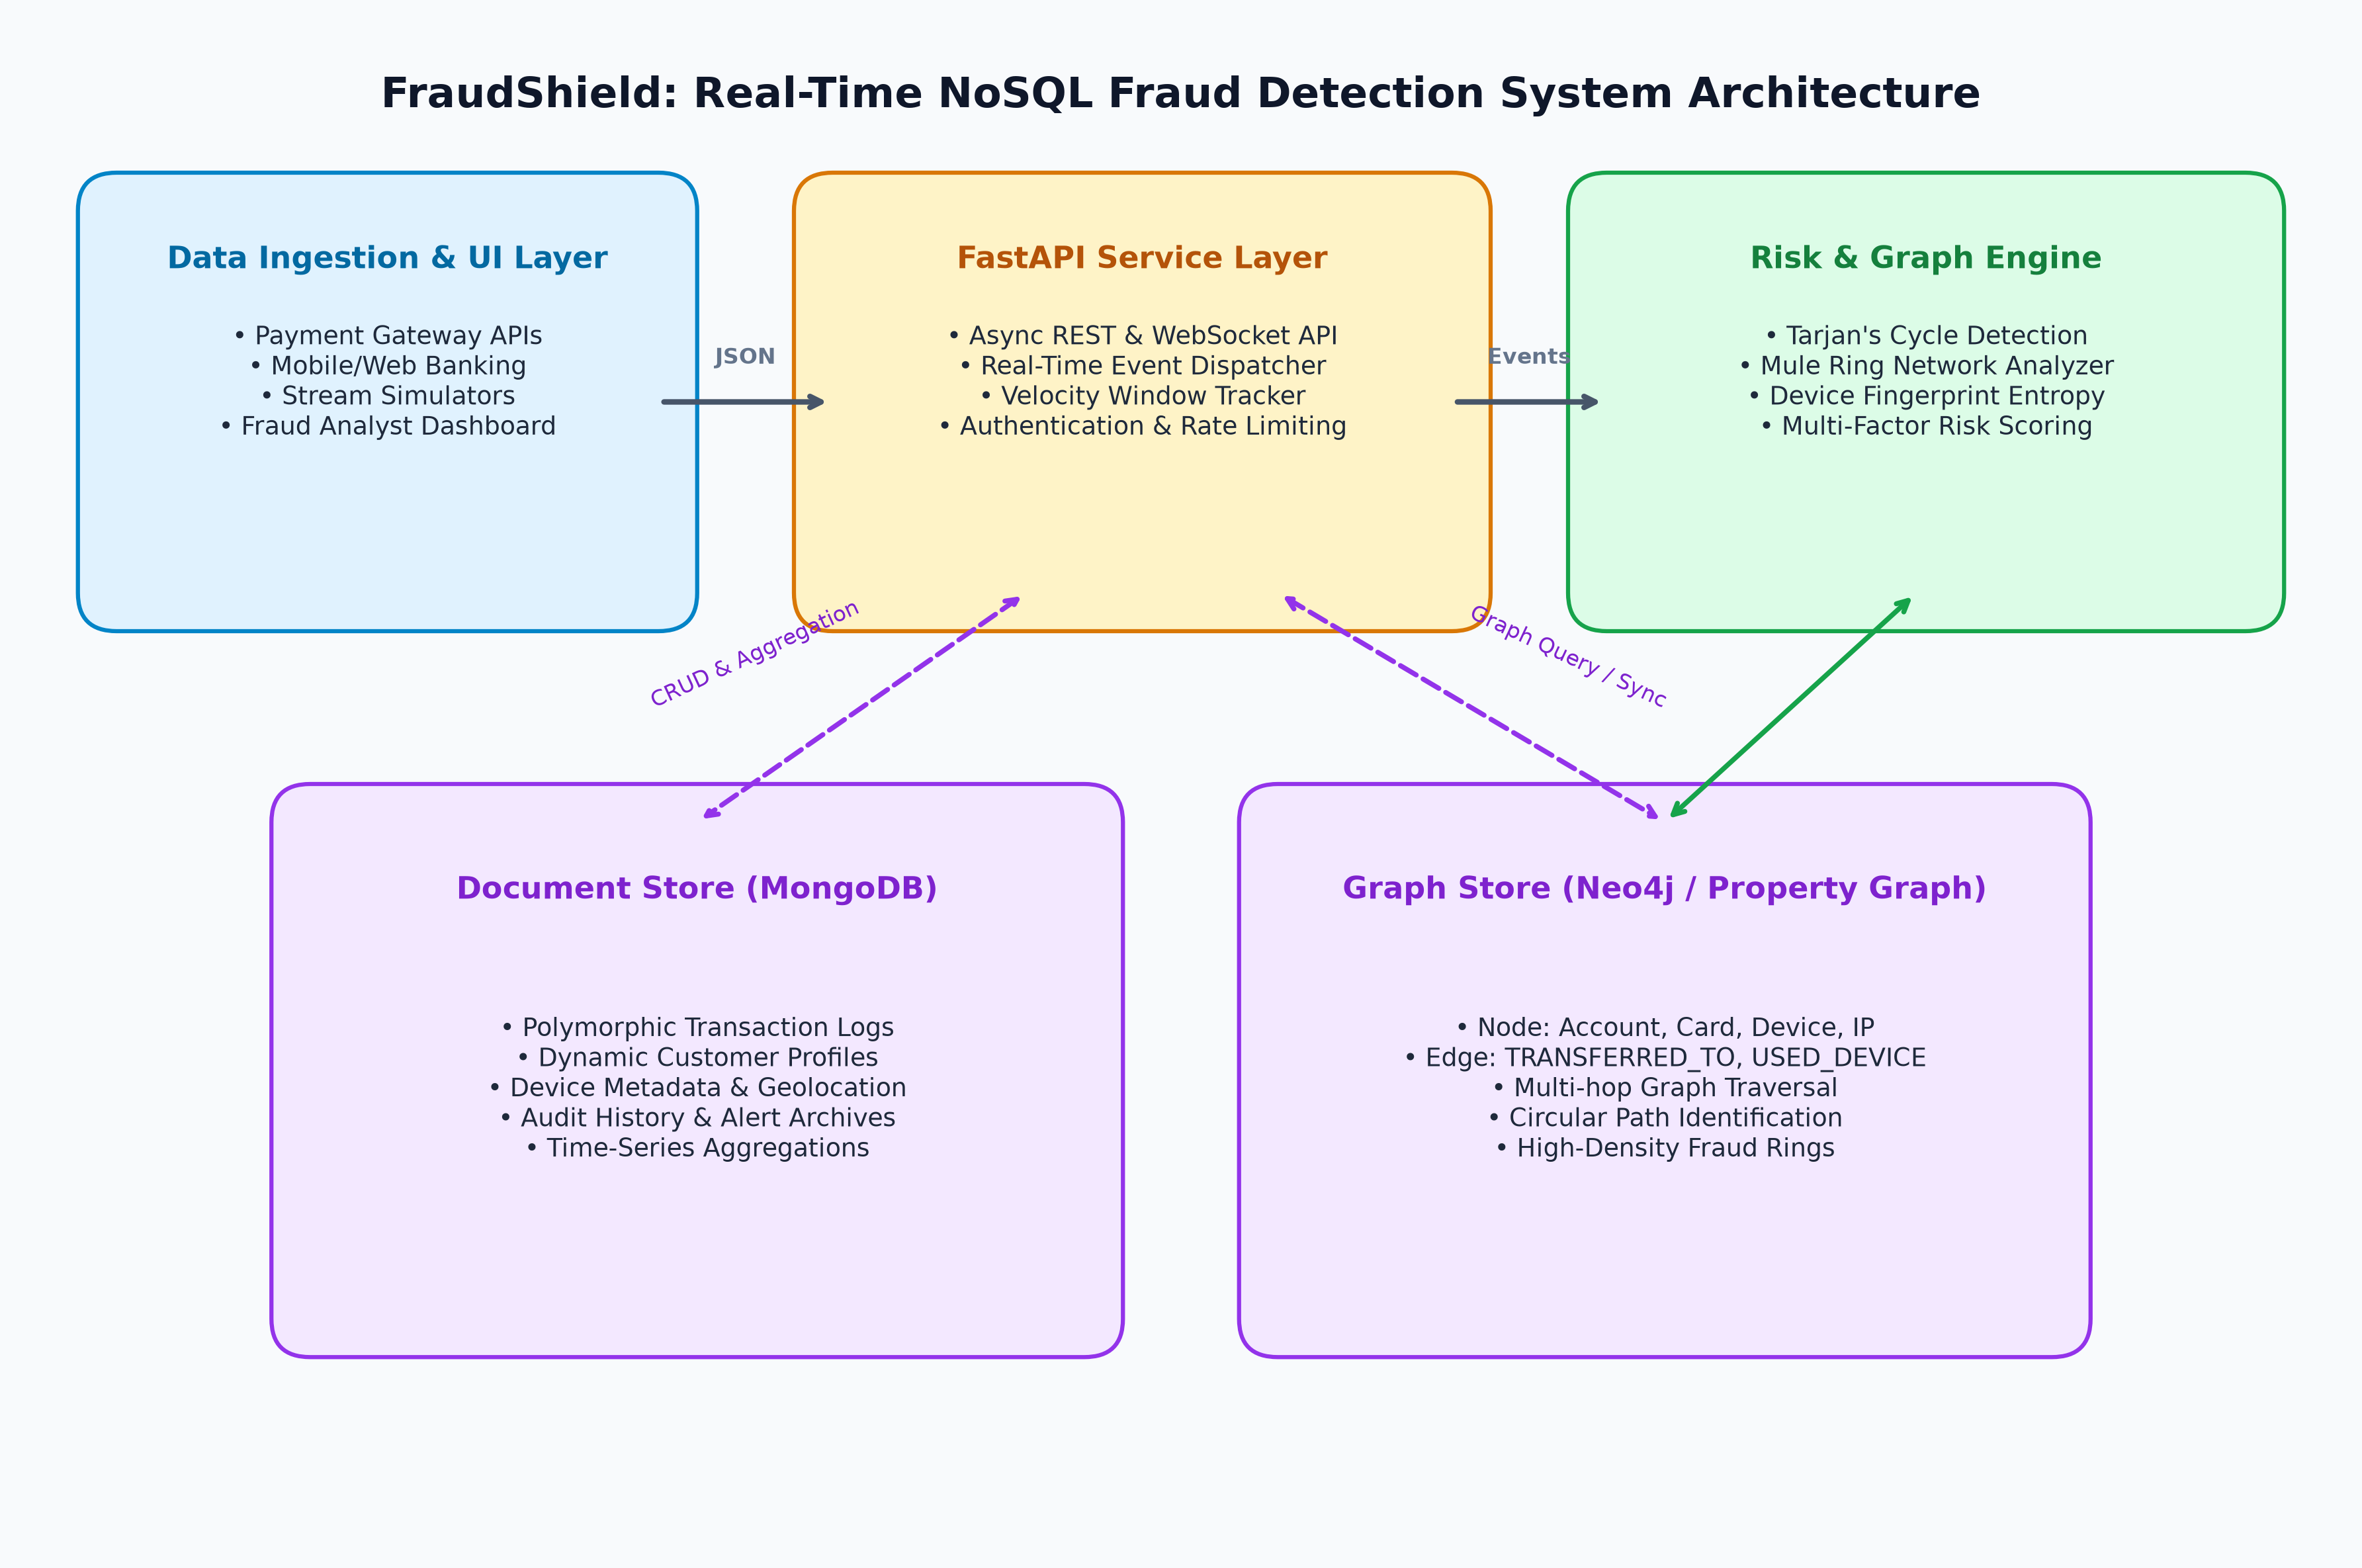
\includegraphics[width=0.88\textwidth]{diagrams/system_architecture.png}
\end{center}

\subsection*{2. Database / Data Model Diagram}
\begin{center}
    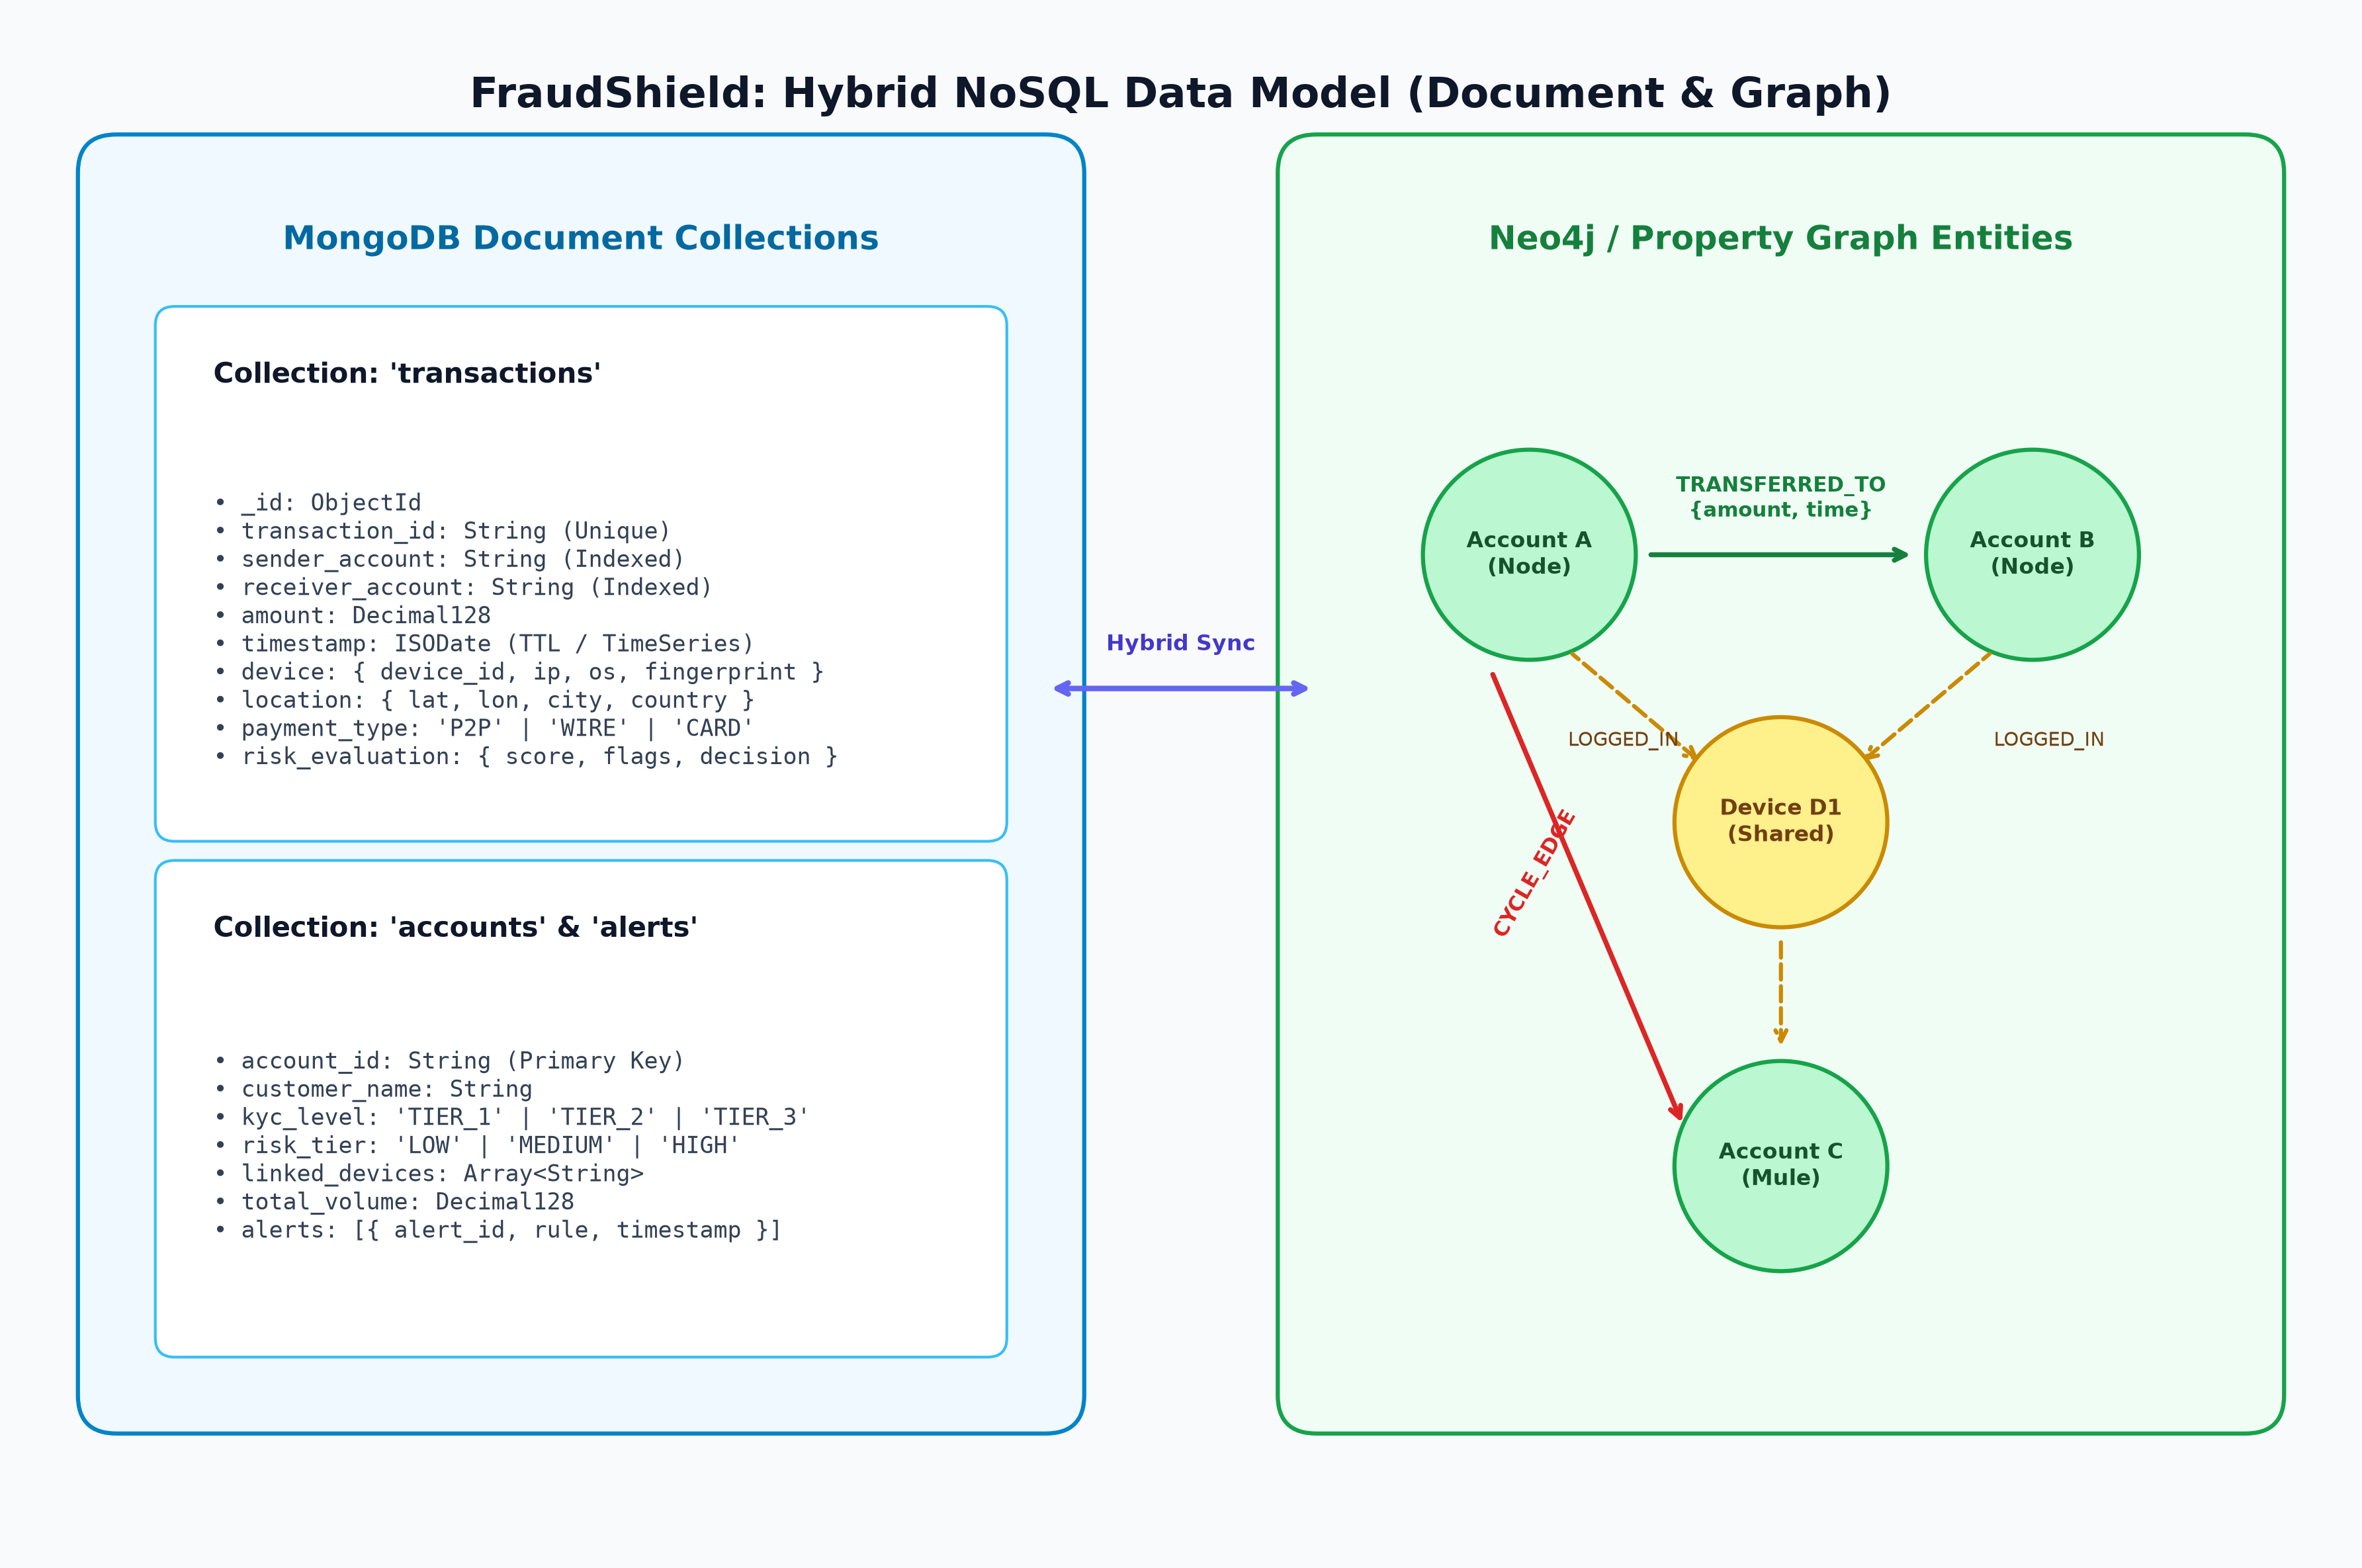
\includegraphics[width=0.88\textwidth]{diagrams/database_data_model.png}
\end{center}

\subsection*{3. Project Workflow / Flowchart}
\begin{center}
    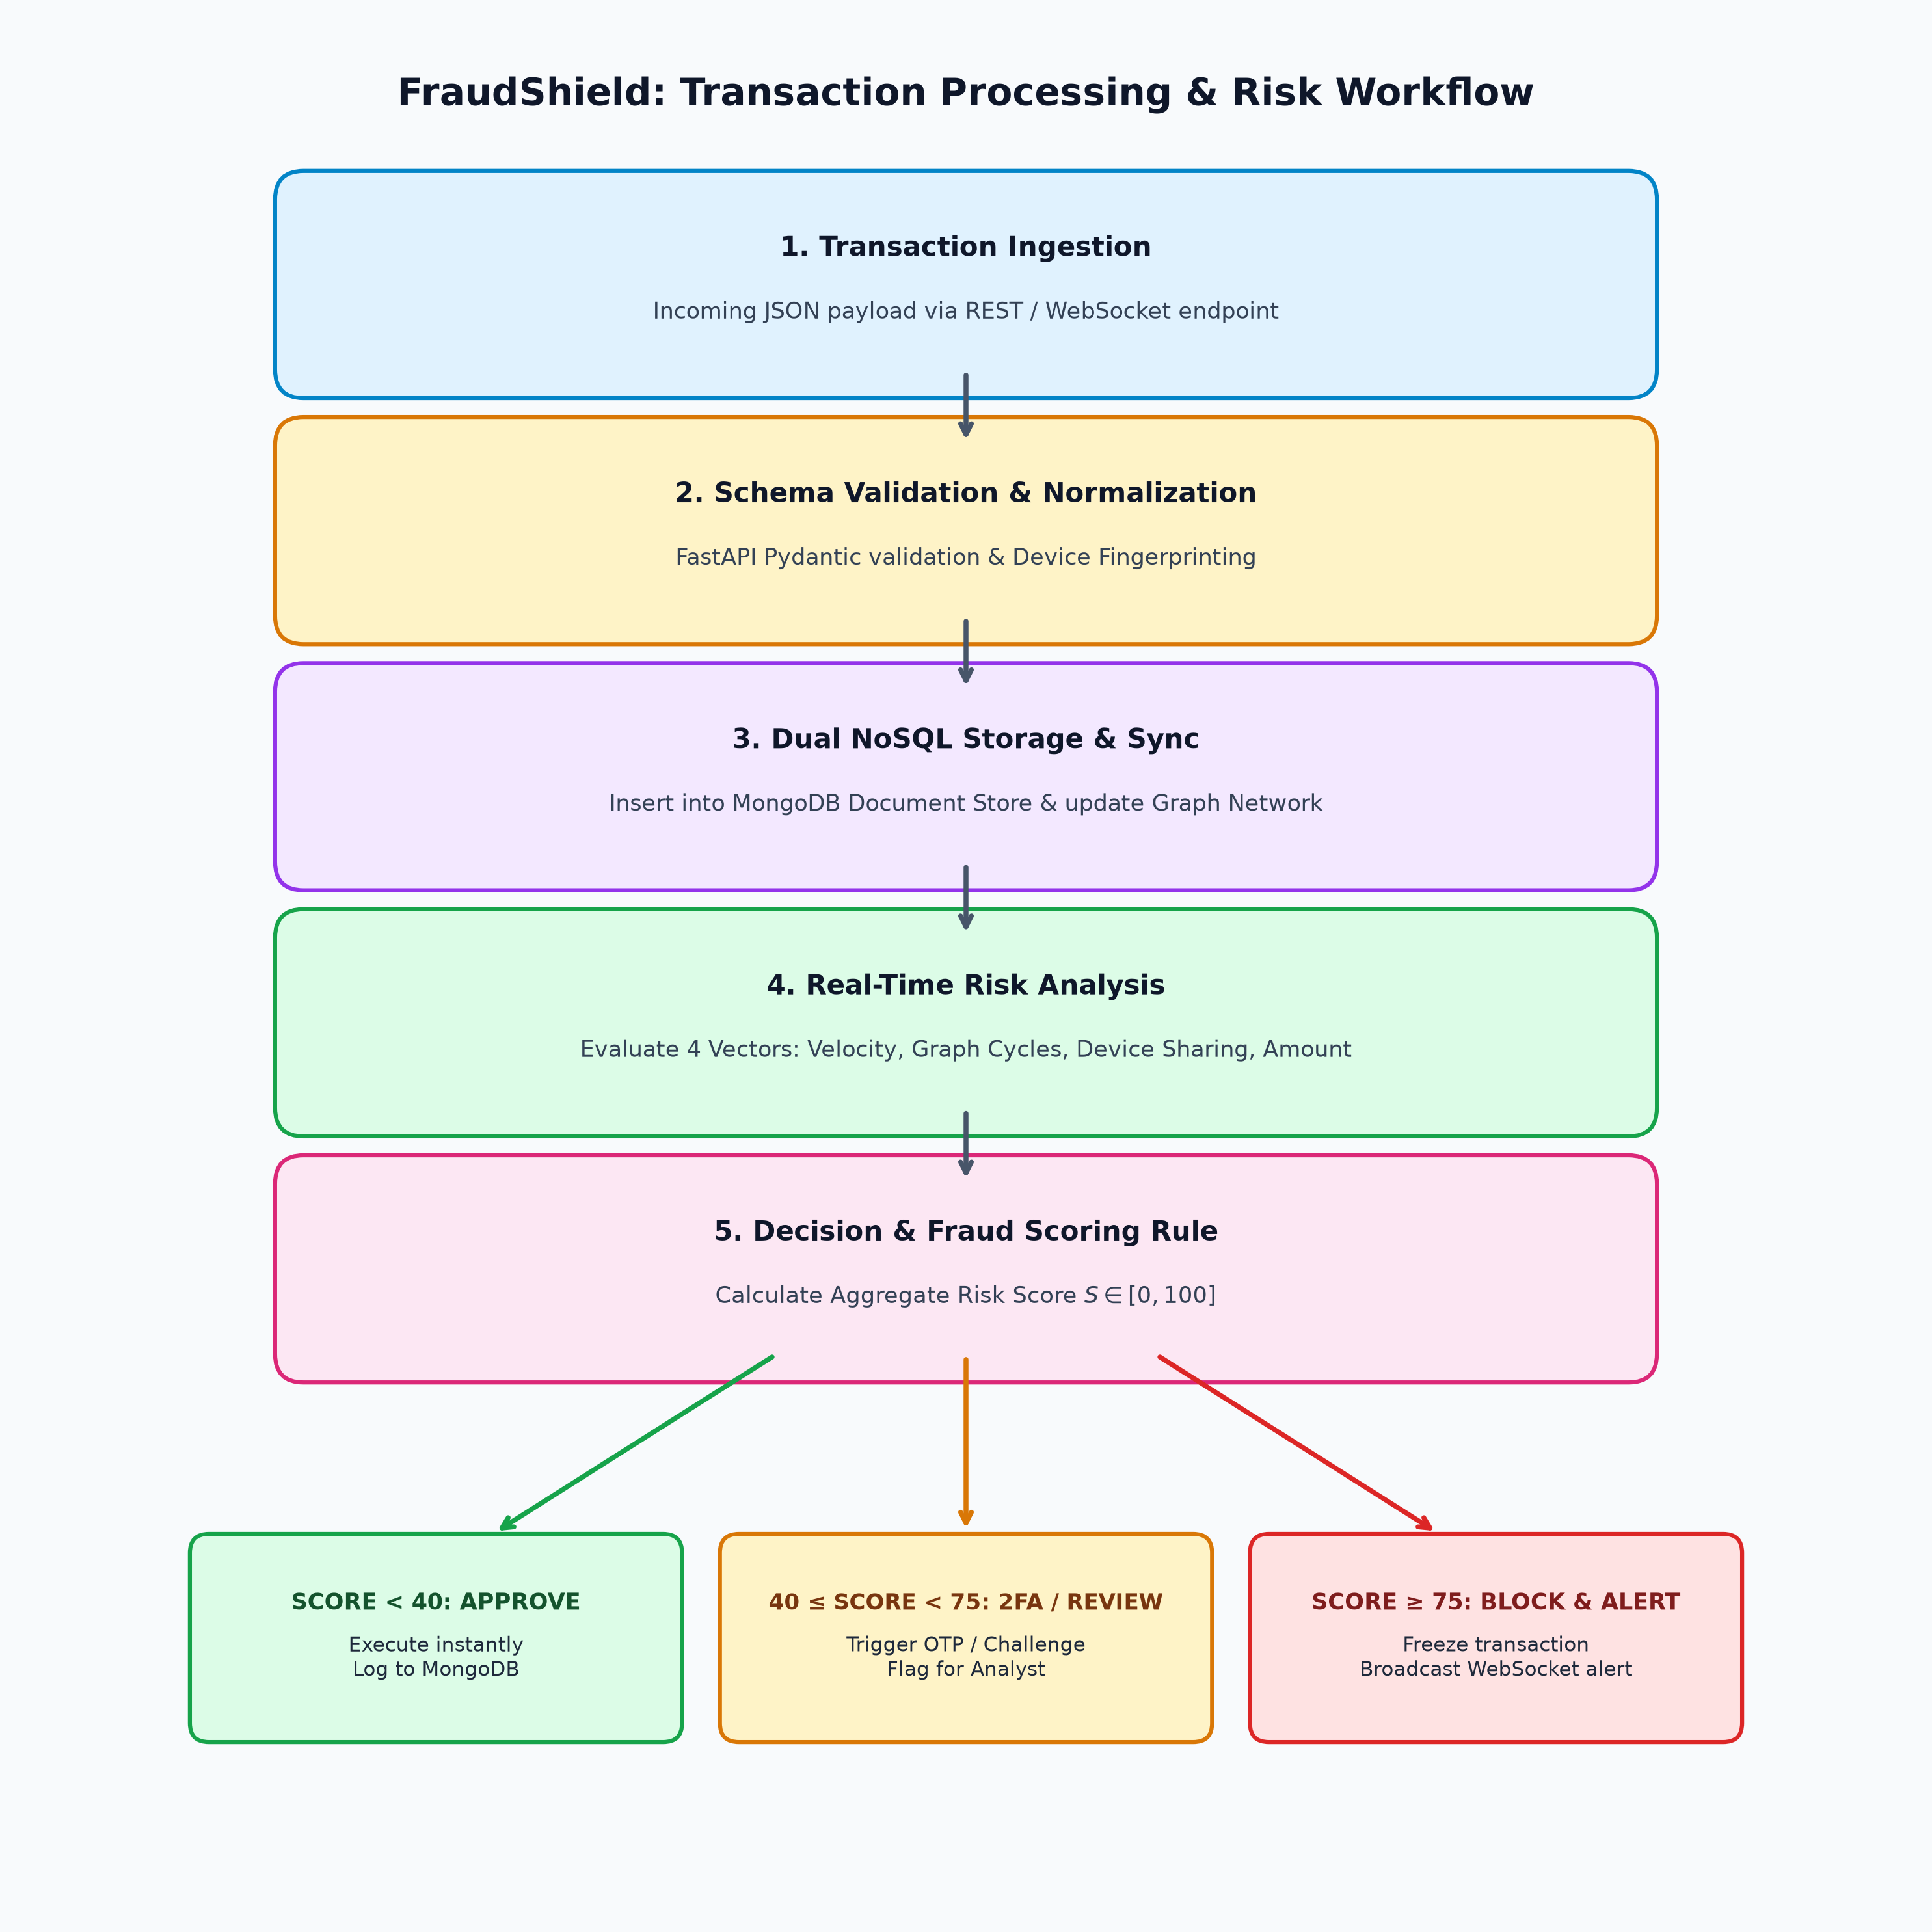
\includegraphics[width=0.72\textwidth]{diagrams/workflow_flowchart.png}
\end{center}

% -------------------------------------------------------------
\newpage
\section{Algorithm / Pseudocode}

\begin{lstlisting}[language=Python, caption={Real-Time Multi-Factor Fraud & Graph Ring Evaluation}]
Algorithm: EvaluateTransactionRisk(Transaction T)
Input: T = {tx_id, sender, receiver, amount, timestamp, device_id, ip}
Output: RiskReport = {risk_score, classification, reasons}

1:  RiskScore <- 0, AnomalyReasons <- []
2:  MongoDB.InsertRecord("transactions", T)
3:  GraphEngine.AddNodesAndEdges(T.sender, T.receiver, T.device_id, T.amount)
4:  
5:  // Step 1: Depth-bounded Graph Cycle Traversal
6:  CyclePath <- GraphEngine.FindDirectedCycle(T.receiver, T.sender, MaxDepth=5)
7:  if CyclePath != EMPTY then
8:      RiskScore <- RiskScore + 45
9:      Append "Circular fraud ring detected: " + CyclePath to AnomalyReasons
10: end if
11: 
12: // Step 2: Shared Device Cluster Analysis
13: SharedAccounts <- GraphEngine.GetSharedDeviceAccounts(T.device_id)
14: if Length(SharedAccounts) >= 3 then
15:     RiskScore <- RiskScore + 30
16:     Append "High-risk device sharing across multiple accounts" to AnomalyReasons
17: end if
18: 
19: // Step 3: MongoDB Sliding-Window Velocity Aggregation
20: BurstCount <- MongoDB.CountVelocity(T.sender, Window="5m")
21: if BurstCount >= 5 then
22:     RiskScore <- RiskScore + 25
23:     Append "Burst transaction velocity spike" to AnomalyReasons
24: end if
25: 
26: if T.amount > 50000.00 then
27:     RiskScore <- RiskScore + 15
28: end if
29: 
30: RiskScore <- Min(100, RiskScore)
31: Decision <- (RiskScore >= 75 ? "HIGH_RISK_BLOCK" : 
                 (RiskScore >= 40 ? "MEDIUM_RISK_2FA" : "LOW_RISK_APPROVE"))
32: return { risk_score: RiskScore, classification: Decision, reasons: AnomalyReasons }
\end{lstlisting}

\vspace{1.5em}
\hrule
\vspace{1em}

\subsection*{Signatures \& Submission Details}

\noindent \textbf{Student Signature:} \underline{\hspace{6cm}} \hfill \textbf{Date:} September 25, 2026\\[1.5em]

\begin{table}[h!]
\centering
\small
\renewcommand{\arraystretch}{1.3}
\begin{tabularx}{\textwidth}{|c|p{3.5cm}|p{3.5cm}|c|c|X|}
\hline
\textbf{S.No.} & \textbf{Name} & \textbf{Print Name} & \textbf{Gender} & \textbf{Nationality} & \textbf{Address} \\ \hline
1. & Sarthak Gupta & Sarthak Gupta & Male & Indian & Jaipur \\ \hline
\end{tabularx}
\end{table}

\end{document}
